\documentclass[aspectratio=169]{beamer}
%\setbeameroption{show notes}

\usepackage{beamer_pre}


\title{Thesis meeting 2024/03/20}
\author{Albert R. S. Garde}
\date{\today}
	

\begin{document}

\frame{
	\maketitle
}

\frame{
	\frametitle{Progress since last meeting}
    \begin{itemize}
        \item Thought a lot about the statistics.
        \item Fixed the last critical bugs in the N2G code.
        \item Ran N2G on the SAE features.
        \item Calculated p-values for the mean of the recall, precision and F1-scores being equal.
    \end{itemize}
}
\frame{
    \frametitle{Plan for the next weeks}
    \begin{itemize}
        \item Look for better way to handle issue with many SAE feature models predicting no fires.
        \item Start work on training own SAEs, since this is necessary for testing the hypothesis more broadly.
        \item Continue work on improving N2G code.
    \end{itemize}
}
\frame{
    \frametitle{Topics for meeting}
    \begin{itemize}
        \item Showcase statistics done.
        \item How to handle NaN values?
        \item Broader thoughts on statistics.
    \end{itemize}
}
\frame{
    \frametitle{Results}
    \begin{table}[h]
        \centering
        \caption{NaN adjusted statistical comparison of N2G models of MLP and SAE features.}
        \label{tab:stat_results}
        \begin{tabular}{lccccc}
        \toprule
         & \multicolumn{2}{c}{\textbf{MLP}} & \multicolumn{2}{c}{\textbf{SAE}} &  \\
        \cmidrule(lr){2-3} \cmidrule(lr){4-5}
         & Mean & SD & Mean & SD & \textbf{$p$-value} \\
        \midrule
        Recall & $0.617$ & $0.0057$ & $0.751$ & $0.0041$ & $0.0053$ \\
        Precision & $0.6451$ & $0.0081$ & $0.7329$ & $0.0040$ & $0.0189$ \\
        F1-score & $0.4749$ & $0.0057$ & $0.6871$ & $0.0040$ & $0.0021$ \\
        \bottomrule
        \end{tabular}
    \end{table}
}
\frame{
    \frametitle{Recall distribution}
    \begin{figure}
        \centering
        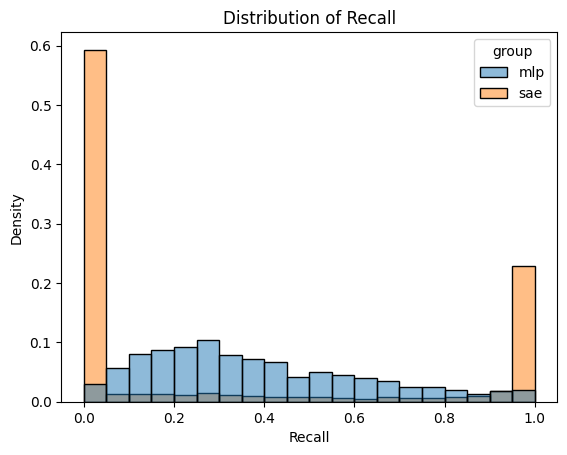
\includegraphics[width=0.6\textwidth]{figures/recall_all.png}
        \caption{Distribution of recall scores for the MLP and SAE models.}
        \label{fig:recall_dist}
    \end{figure}
}
\frame{
    \frametitle{Non NaN distributions}
    \begin{figure}
        \centering
        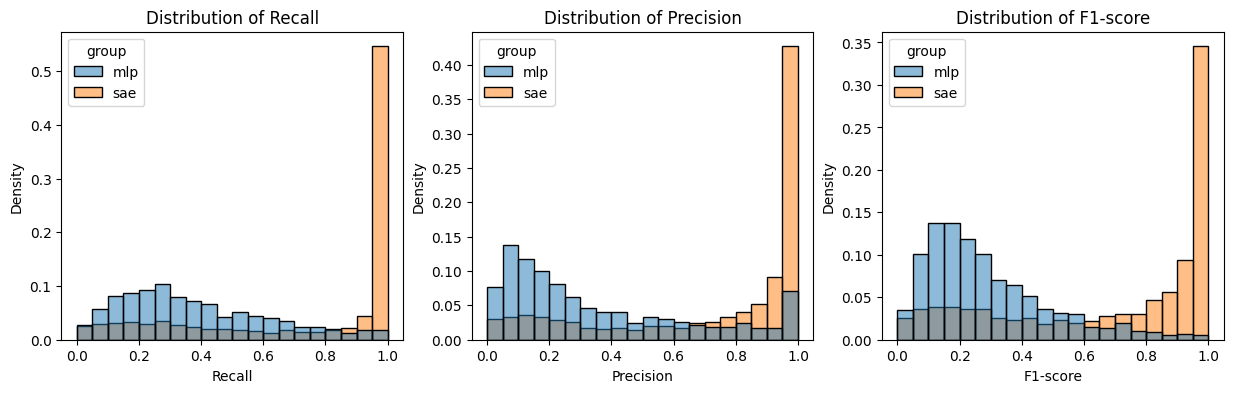
\includegraphics[width=1\textwidth]{figures/all_notnull.png}
        \caption{Distribution of non NaN scores.}
        \label{fig:all_dist_notnull}
    \end{figure}
}

\end{document}